\chapter{Created Visualizations}
This section of the included appendix contains several figures visualizing the user and item vectors produced by the implemented recommenders. All visualizations were made using the TensorFlow Embedding Projector \footnote{Available at: \url{https://projector.tensorflow.org/}}, an online tool for visualizing high-dimensional data. All files needed to perform these visualizations are prepared in the \texttt{data/visualization} folder and therefore can be used once again with the embedding projector to inspect the created vectors and further experiment with them.

\begin{figure}[H]
    \centering
    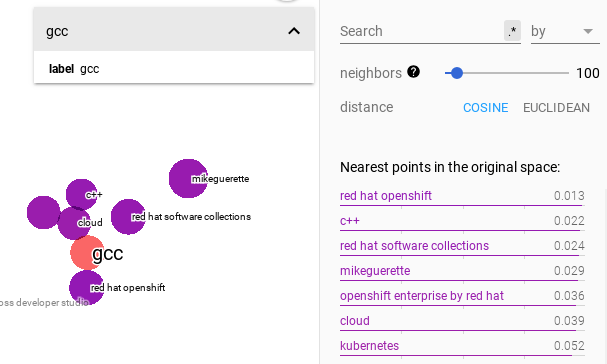
\includegraphics[scale=0.6]{obrazky-figures/tags_2.png}
    \caption{Visualization of the tag embeddings learned by \texttt{SkipGramRecommender}. During its training, the model is learning not only the weights of its hidden layer but also its tag embeddings. This figure shows tags that were positioned close to the tag \texttt{gcc} in the created space. The correctness of the visualized embeddings could be questioned, however, it is safe to say that at least the \texttt{gcc} and \texttt{c++} tags make sense to be positioned close to each other.}
\end{figure}


\begin{figure}[H]
    \centering
    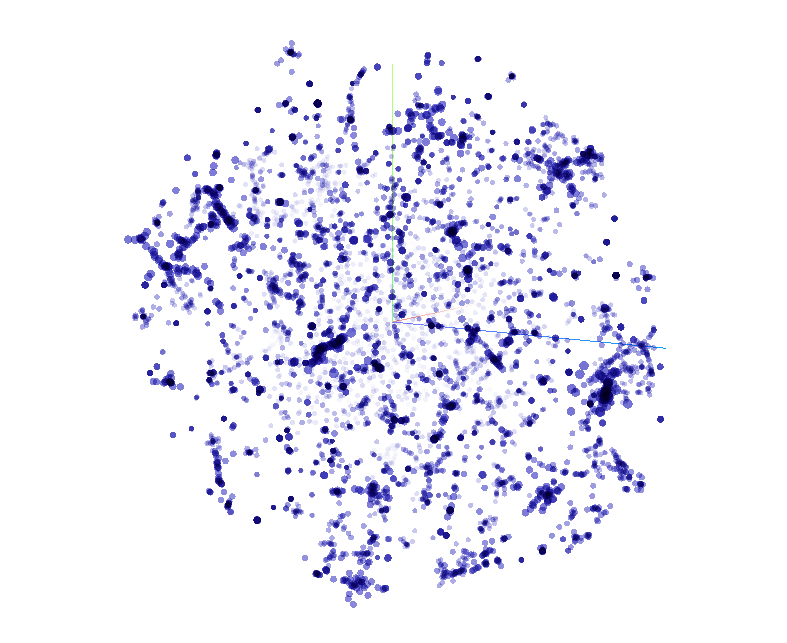
\includegraphics[scale=0.43]{obrazky-figures/svd_uid.png}
    \caption{Visualization of the matrix U created by the \texttt{SVD} recommender. Matrix U consists of vectors representing the latent features of users. The figure shows several small clusters emerging across the original space.}
    \label{ap:svd_u}
\end{figure}

\begin{figure}[H]
    \centering
    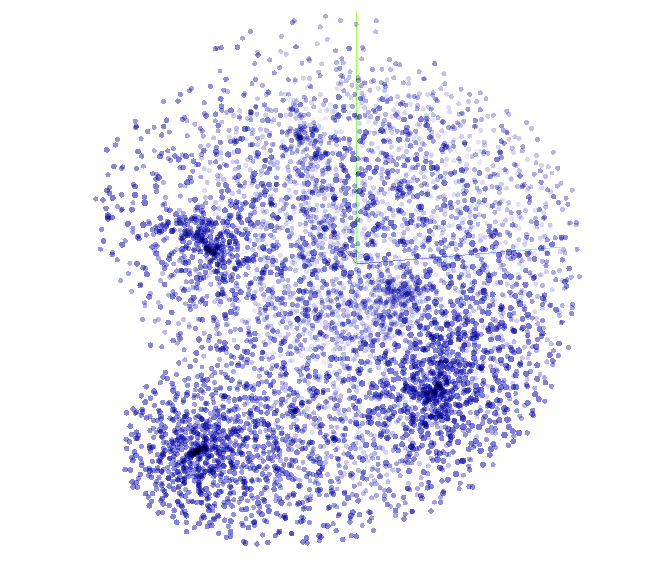
\includegraphics[scale=0.43]{obrazky-figures/als2.png}
    \caption{Visualization of user vectors created by the \texttt{ALS} recommender. Opposed to figure \ref{ap:svd_u}, here the emerging clusters are denser and less frequent.}
\end{figure}


\begin{figure}[H]
    \centering
    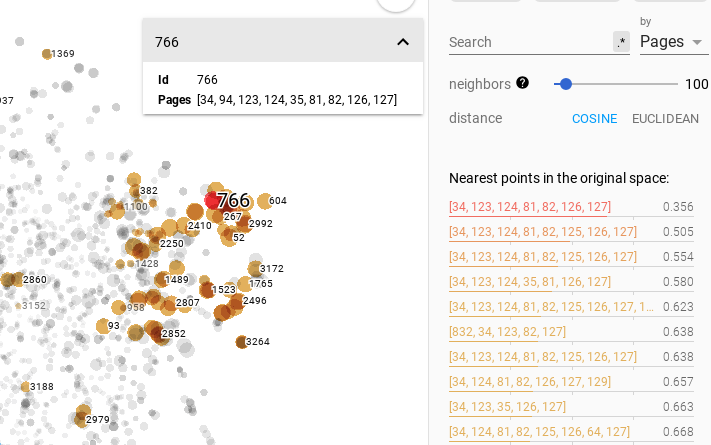
\includegraphics[scale=0.55]{obrazky-figures/svd_uid2.png}
    \caption{Detailed image of matrix U from figure \ref{ap:svd_u}. It shows a user, identified by id=766 and a list of items he interacted with, also represented by their integer ids. On the right side, it shows the nearest users to user 766, represented by lists of their items. Items 34, 123, 124 and several others can be found in most of the lists, which means that the model managed to correctly place similar users close to each other.}
    \label{ap:svd_detail}
\end{figure}

\begin{figure}[H]
    \centering
    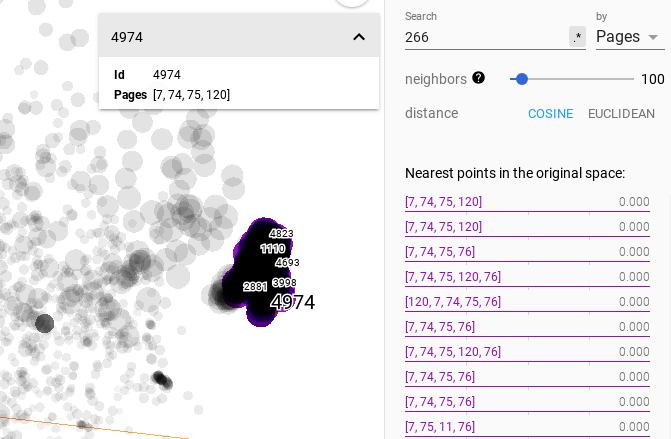
\includegraphics[scale=0.55]{obrazky-figures/als_similarities.png}
    \caption{Similarly, as in figure \ref{ap:svd_detail}, this figure shows the most similar users of a user vector created by the \texttt{ALS} recommender. Again it is clear that in this particular case the model managed to correctly place users with similar items close to each other.}
\end{figure}


\begin{figure}[H]
    \centering
    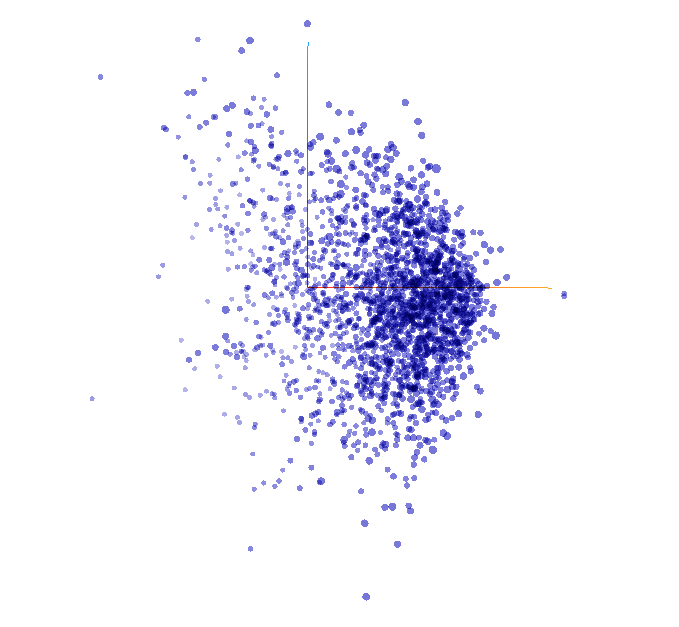
\includegraphics[scale=0.43]{obrazky-figures/doc2vec_local2.png}
    \caption{The locally trained 13-dimensional document vectors, created by the \texttt{Doc2Vec} recommender.}
    \label{ap:doc2vec_local}
\end{figure}

\begin{figure}[H]
    \centering
    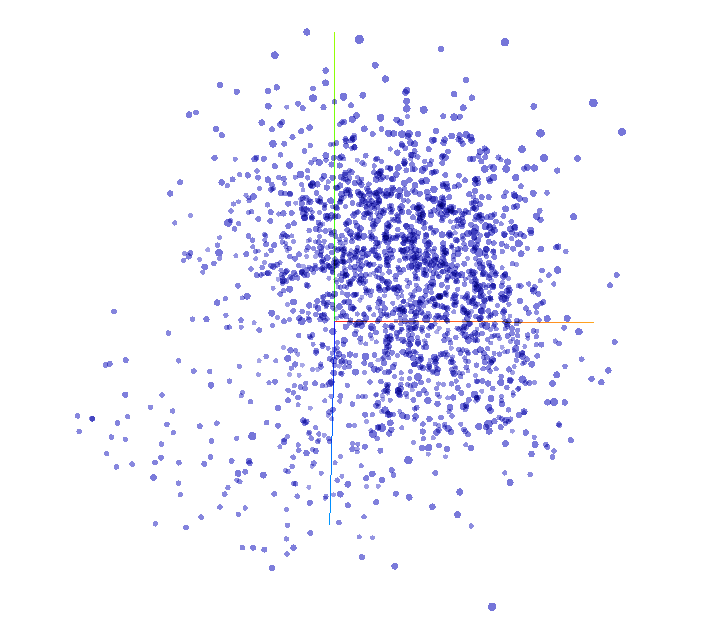
\includegraphics[scale=0.43]{obrazky-figures/doc2vec_wiki.png}
    \caption{Document vectors created using the pre-trained 300-dimensional model by the \texttt{Doc2Vec} recommender.}
\end{figure}


\begin{figure}[H]
    \centering
    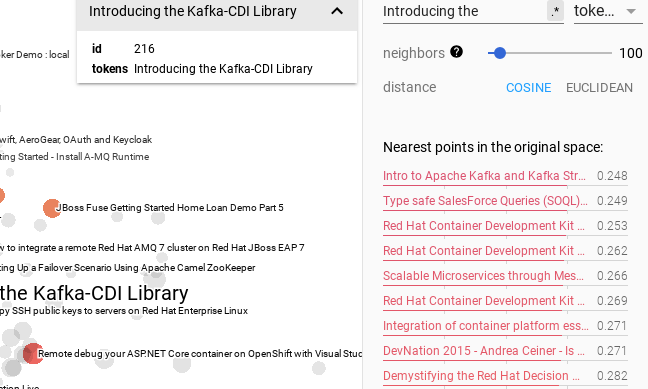
\includegraphics[scale=0.58]{obrazky-figures/doc2vec_local5.png}
    \caption{Finding the nearest items with the locally trained \texttt{Doc2Vec} recommender \ref{ap:doc2vec_local}. The tokens value contains the title of each article.}
    \label{ap:doc2vec_local_detail}
\end{figure}

\begin{figure}[H]
    \centering
    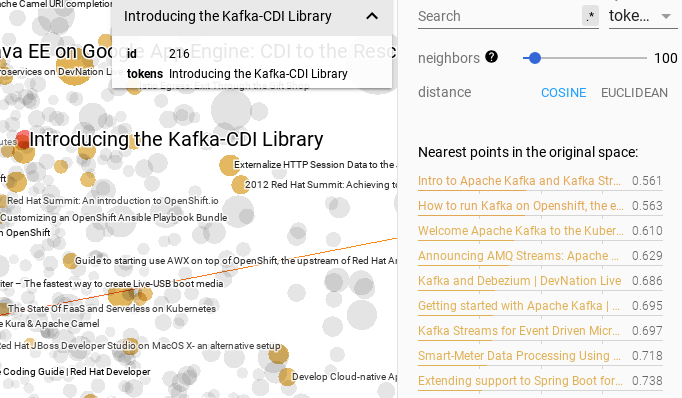
\includegraphics[scale=0.58]{obrazky-figures/doc2vec_wiki3.png}
    \caption{Finding the nearest items using the pre-trained Doc2Vec recommender. This figure shows the same item as figure \ref{ap:doc2vec_local_detail}. The comparison is in favour of the pre-trained model as it appears to show more relevant items.}
\end{figure}


\chapter{Contents of the enclosed DVD}
The DVD enclosed as part of this thesis consists of the following tree structure: \\

\dirtree{%
    .1 /.
    .2 data.
    .3 json \quad \ldots{} \begin{minipage}[t]{10cm}
                        Directory with articles metadata
                \end{minipage}.
    .3 processed \ldots{} \begin{minipage}[t]{10cm}
                        Directory with the processed dataset
                \end{minipage}.
    .3 visualizing \ldots{} \begin{minipage}[t]{10cm}
                        Directory containing user and item vectors saved for visualizations \\
                \end{minipage}.
    .2 src \quad \ldots{} \begin{minipage}[t]{10cm}
                        Contains all models and other source files
                \end{minipage}.
    .3 svd$\_$model{.}py.
    .3 als$\_$model{.}py.
    .3 doc2vec$\_$class{.}py.
    .3 doc2vec$\_$model{.}py.
    .3 skipgram$\_$model{.}py.
    .3 evaluation{.}py.
    .3 optimization{.}py.
    .3 optimal$\_$parameters{.}py \\.
    .2 src\_doc \ldots{} \begin{minipage}[t]{10cm}
                        Directory containing all source files of the latex documentation
                \end{minipage}.
    .2 doc \quad \ldots{} \begin{minipage}[t]{10cm}
                        Contains this pdf file \\
                \end{minipage}.
    .3 thesis{.}pdf \\.
    .2 README{.}md.
    .2 requirements{.}txt \ldots{} \begin{minipage}[t]{10cm}
                        File containing all required libraries
                \end{minipage}.
}